% !TeX root =  main.tex

\chapter{Sequences and Series}

\section{Sequences}

\begin{definition}[Definition of a Sequence]
A sequence is a function $a$ whose domain is the set of natural numbers. The terms of the sequence are the function values $a(1)$, $a(2)$, $a(3)$, $\cdots$, $a(n)$, $\cdots$
We usually write $a_n$ instead of the function notation $a(n)$. So the terms of the sequence are written as
$a_1$, $a_2$, $a_3$, $\cdots$, $a_n$, $\cdots$
The number $a_1$ is called the first term,$a_2$ is called the second term,and in general,$a_n$ is called the $n$-th term.
\end{definition}
\begin{example}
    Find the first five terms and the 100-th term of the sequence defined by each formula.\\
    \begin{enumerate*}
        \item $a_n=2n-1$
        \item $c_n=n^2-1$
        \item $t_n=\dfrac{n}{n+1}$
        \item $r_n=\dfrac{(-1)^n}{2^n}$\hfill\null
    \end{enumerate*}
\end{example}

\begin{example}
    Find the $n$-th term of a sequence whose first several terms are given.
    \begin{enumerate}
        \item $\frac{1}{2}$, $\frac{3}{4}$, $\frac{4}{5}$, $\frac{5}{6}$, $\cdots$
        \item $\frac{1}{2}$, $\frac{3}{4}$, $\frac{5}{6}$, $\frac{7}{8}$, $\cdots$
        \item $-2$, $4$, $-8$, $16$, $\cdots$
        \item $2$, $5$, $8$, $11$, $\cdots$
    \end{enumerate}
\end{example}

\newpage

\begin{definition}
  In some sequences, the $n$-th term may depend on some or all of the terms preceding it. Such a sequence is called \textbf{recursive sequence}.  
\end{definition}

\begin{example}
   A sequence is defined recursively by $a_1=1$ and $a_n=3(a_{n-1}+2)$.
   \begin{enumerate}
       \item Find the first five terms of the sequence.
       \item Find the first five terms of the sequence $\{b_n\}$ where $b_n=a_n-a_{n-1}$.
       % \item \xout{Find the $n$-th term of $b_n$.}
       % \item \xout{Find the $20$-th term of $a_n$.}
       % \item \xout{Find the $n$-th term of $a_n$.}
   \end{enumerate}
\end{example}

\begin{example}[The Fibonacci Sequence]
    Find the first 11 terms of the sequence defined recursively by $F_1=1$, $F_2=1$ and 
    $$F_n=F_{n-1} + F_{n-2}.$$
\end{example}


\newpage
\begin{definition}[The Partial Sums of a Sequence]
For the sequence $\{a_n\}$, the sum $S_n$ for first $n$ terms is called the $n$-th partial sum. The sequence $\{S_n\}$ is called the sequence of partial sums.
\end{definition}


\begin{example}
    Find the first four partial sums and the $n$-th partial sum of the sequence given by $a_n=\dfrac{1}{2^n}$.
\end{example}


\begin{example}
    Find the first four partial sums and the $n$-th partial sum of the sequence given by $a_n=\dfrac{1}{n}-\dfrac{1}{n+1}$.
\end{example}

\newpage

\begin{definition}[Sigma notation]
    The sigma notation or summation notation for a partial sum of the first $n$-terms of a sequence $a_n$ is defined as
    \[\sum_{k=1}^na_k.\]
    The left side is read as ``the sum of $a_k$ from $k=1$ to $k=n$".  The letter
$k$ is called the index of summation, or the summation variable.
\end{definition}

\begin{example}
    Find the sum.\\
    \begin{enumerate*}
        \item $\sum\limits_{k=1}^5 k^2$
        \item $\sum\limits_{j=3}^5\dfrac{1}{j}$\hfill\null
    \end{enumerate*}
\end{example}

\begin{example}
    Write each sum using sigma notation.\\
    \begin{enumerate*}
        \item $1^3+2^3+4^3+\cdots+7^3$
        \item $\sqrt{1}+\sqrt{3}+\sqrt{5}+\cdots+\sqrt{13}$\hfill\null
    \end{enumerate*}
\end{example}

\begin{theorem}[Properties of sums] Let $\{a_n\}$ and $\{b_n\}$ be two sequences.
    \begin{enumerate}
        \item $\sum\limits_{k=1}^n (c\cdot a_k+ d\cdot b_k)=c\sum\limits_{k=1}^n a_k+d\sum\limits_{k=1}^nb_k$ for any constants $c$ and $d$.
        \item $\sum\limits_{k=1}^na_k=\sum\limits_{k=1}^m a_k +\sum\limits_{k=m+1}^n$ for any $1<m<n$.
    \end{enumerate}
\end{theorem}

\newpage

\section*{Exercises}

\begin{exercise}
    Find the first 12-th terms of the sequence with the given $n$-th term.\\
\begin{enumerate*}
    \item $a_n=\dfrac{n^2}{n+1}$
    \item $a_n=(-1)^n\dfrac{2^n}{n}$
    \item $a_n=\dfrac{(2n)!}{2^nn!}$\hfill\null
\end{enumerate*}
\end{exercise}

\begin{exercise}
    Find the first nine terms of the sequence.
\begin{enumerate}
    \item $a_n=a_{n-1}+2n-1$, $a_1=1$
    \item $a_n=(-1)^n\dfrac{a_{n-1}}{n}$, $a_1=1$
    \item $a_n=a_{n-1}-a_{n-2}$, $a_1=1$ and $a_2=2$
\end{enumerate}
\end{exercise}

\newpage

\begin{exercise}
  Find the sum.\\
  \begin{enumerate*}
      \item $\sum\limits_{k=1}^4 k^3$
      \item $\sum\limits_{j=2}^4\dfrac{1}{j-1}$\hfill\null
  \end{enumerate*}
\end{exercise}

\begin{exercise}
  Write each sum using sigma notation.\\
  \begin{enumerate*}
      \item $1^3+3^3+5^3+\cdots+11^3$
      \item $\sqrt[3]{1}+\sqrt[3]{2}+\sqrt[3]{3}+\cdots+\sqrt[3]{10}$\hfill\null
  \end{enumerate*}
\end{exercise}

\begin{exercise}
  Find the partial sum.\\
  \begin{enumerate*}
      \item $\sum\limits_{k=1}^{10}(k-1)^2$
      \item $\sum\limits_{i=2}^{7}\dfrac{2i}{2i-1}$
      \item $\sum\limits_{j=1}^{3}\dfrac{(-2)^j}{j+1}$\hfill\null
  \end{enumerate*}
\end{exercise}

\newpage

\section{Arithmetic Sequences}

\begin{definition}
 An arithmetic sequence is a sequence of the form
\[a, a+d, a+2d, a+3d, a+4d, \cdots\]
The number $a$ is the first term, and $d$ is the common difference of the sequence. The $n$-th term of an arithmetic sequence is given by
\[a_n=a+(n-1)d.\]
\end{definition}

\begin{example}
    Find $a_n$ for the arithmetic sequence
    \[9,4,-1,-6,-11,\cdots\]
\end{example}

\begin{example}
The 11-th term of an arithmetic sequence is 32, and the 19-th term is 72. Find the 100-th term.
\end{example}

% \noindent
% \begin{minipage}{\textwidth}
%  \begin{minipage}{0.49\textwidth}
        \begin{theorem}[Sum of natural numbers]\mbox{}
    \begin{enumerate}
        \item $\sum\limits_{k=1}^n c=cn$, where $c$ is a constant.
        \item $\sum\limits_{k=1}^n k=\dfrac{n(n+1)}{2}$.
    \end{enumerate}
\end{theorem}
%     \end{minipage}
%     \begin{minipage}{0.49\textwidth}
%         \centering
% 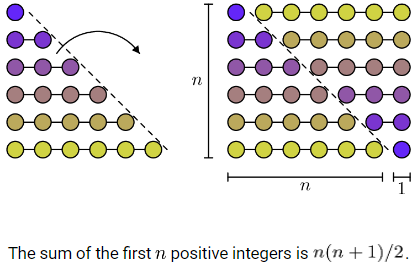
\includegraphics[width=0.6\textwidth, keepaspectratio]{figs/sumofk.png}
%     \end{minipage}
% \end{minipage}

\newpage

\begin{theorem}[Sum of an Arithmetic Sequence]
    For the \textbf{arithmetic sequence} $a_n$, the $n$-th partial sum is
    \[S_n=\sum\limits_{k=1}^n a_k=n\left(\dfrac{a_1+a_n}{2}\right).\]
\end{theorem}

\begin{example}
    Find the sum of the first 50 odd numbers.
\end{example}

\begin{example}
    Find the following partial sum of an arithmetic sequence:
    \[3+7+11+15+\cdots+159.\]
\end{example}

\begin{example}
    How many terms of the arithmetic sequence $5$, $7$, $9$, $\cdots$ must be added to get $572$?
\end{example}

% \newpage
% \textbf{The following results are optional.}

% \begin{minipage}{\textwidth}
%     \begin{minipage}{0.4\textwidth}
% \begin{theorem}[Sum of squares]
% \[\sum\limits_{k=1}^n k^2=\dfrac{n(n+1)(2n+1)}{6}.\]
% \end{theorem}
%     \end{minipage}
%     \begin{minipage}{0.55\textwidth}
%         \centering
% 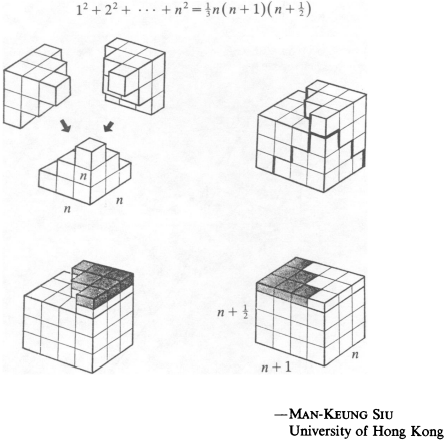
\includegraphics[width=0.54\textwidth, keepaspectratio]{figs/sumsquares.png}
%     \end{minipage}
% A visualization can be found here: 
% \href{Proof without words: Sum of the square - an animation by Daniel Mentrard}{https://www.geogebra.org/m/w6ussdkd}
% \end{minipage}
% \vspace*{\baselineskip}

% \begin{minipage}{\textwidth}
%     \begin{minipage}{0.4\textwidth}
% \begin{theorem}[Sum of cubes]
% \[\sum\limits_{k=1}^n k^3=\dfrac{n^2(n+1)^2}{4}.\]
% \end{theorem}
%     \end{minipage}
%     \begin{minipage}{0.55\textwidth}
%         \centering
% 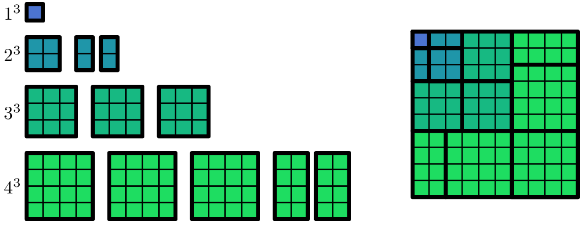
\includegraphics[width=0.54\textwidth, keepaspectratio]{figs/sumcubes.png}
%     \end{minipage}
% \end{minipage}
% \vspace*{\baselineskip}

\newpage

\section*{Exercises}

\begin{exercise}
Find the $n$-th term of the sequence and determine whether the sequence is an arithmetic sequence or not. 
\begin{enumerate}
    \item $1-\sqrt{2}$, $1-2\sqrt{2}$, $1-3\sqrt{2}$, $1-4\sqrt{2}$, $\cdots$
    \item $\sqrt{3}$, $3$, $3\sqrt{3}$, $9$, $\cdots$
    \item $1$, $-\frac{3}{2}$, $2$, $-\frac{5}{2}$, $3$, $\cdots$
\end{enumerate}
\end{exercise}

\begin{exercise}
    Find the partial sum.
    \[\frac13+\frac23+1+\frac43+\frac53+\cdots+33\]
\end{exercise}

\begin{exercise}
  How many terms of the arithmetic sequence $3$, $7$, $11$, $\cdots$ must be added to get $170$?
\end{exercise}

\newpage

\section{Geometric Sequences}

\begin{definition}[Definition of a Geometric Sequence]
A \textbf{geometric sequence} is a sequence of the form
\[a, ar, ar^2, ar^3, ar^4, \cdots.\]
The number $a$ is the first term, and $r$ is the common ratio of the sequence.
The $n$-th term of a geometric sequence is given by
\[a_n=ar^{n-1}.\]
\end{definition}

\begin{example}
    Find $a_n$ for the geometric sequence.\\
    \begin{enumerate*}
        \item $2$, $-10$, $50$, $-250$, $1250$, $\cdots$.
        \item $1$, $\frac{1}{3}$, $\frac{1}{9}$, $\frac{1}{27}$, $\frac{1}{81}$, $\cdots$.\hfill\null
    \end{enumerate*}
\end{example}

\begin{example}
    The third term of a geometric sequence is $\frac{63}{4}$, and the sixth term is $\frac{1701}{32}$. Find the fifth term.
\end{example}

\newpage
\begin{theorem}[Sum of a geometric sequence]
    For the geometric sequence $a$, $a r$, $a r^2$, $a r^3$, $a r^4$, $\dots$, $a r^{n-1}$, $ldots$, the $n$-th partial sum is
$$
S_n=\sum_{k=1}^n a r^{k-1}=\dfrac{a(1-r^n)}{1-r}.
$$
\end{theorem}
% \begin{proof}
% To find a formula for $S_n$, we multiply $S_n$ by $r$ and subtract from $S_n$.
% $$
% \begin{aligned}
% S_n &=a+a r+a r^2+a r^3+a r^4+\cdots+a r^{n-1} \\
% r S_n &=a r+a r^2+a r^3+a r^4+\cdots+a r^{n-1}+a r^n \\
% \hline S_n-r S_n &=a-a r^n
% \end{aligned}
% $$
% So
% $$
% \begin{aligned}
% S_n(1-r) &=a\left(1-r^n\right) \\
% S_n &=\frac{a\left(1-r^n\right)}{1-r} \quad r \neq 1
% \end{aligned}
% $$
% \end{proof}

\begin{example}
    Find the following partial sum of a geometric sequence:
\[1+4+16+\cdots+4096.\]
\end{example}

\begin{example}
    Find the sum 
    \[\sum\limits_{k=1}^67\left(-\frac23\right)^{k-1}.\]
\end{example}

\newpage

\begin{definition}
    An expression of the form
    \[\sum_{k=1}^\infty a_k= a_1 + a_2 + a_3 + a_4 + \cdots\]
is called a infinite series.
\end{definition}

% \begin{example}
% The figure on the left shows the sum of an infinite geometric series $\sum\limits_{k=1}^\infty\frac14\cdot\left(\frac12\right)^k$

% The idea can be used to find the sum of any infinite geometric series $\sum\limits_{k=1}^\infty ar^n$ for $0<r<1$.

% \begin{center}
%     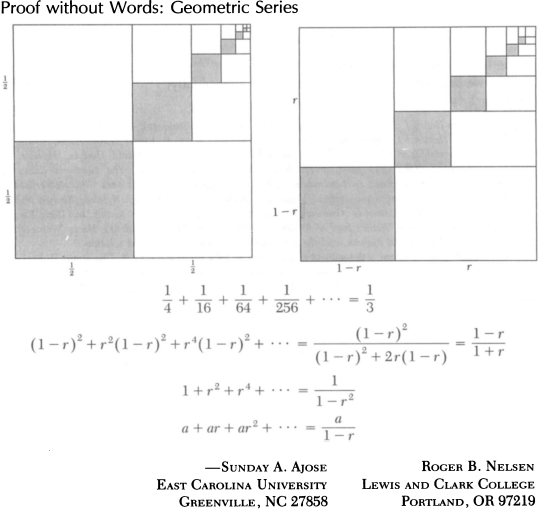
\includegraphics[width=0.8\textwidth]{figs/infiniteseries-arn.png}
% \end{center}
% \end{example}

\begin{theorem}[SUM OF AN INFINITE GEOMETRIC SERIES]
If $|r|<1$, then the infinite geometric series
$$
\sum_{k=1}^{\infty} a r^{k-1}=a+a r+a r^2+a r^3+\cdots
$$
converges and has the sum
$$
S=\frac{a}{1-r}
$$
If $|r| \geq 1$, the series diverges.
\end{theorem}


\begin{example}
Determine whether the infinite geometric series is convergent or divergent. If it is convergent, find its sum.\\
\begin{enumerate*}
  \item $\sum\limits_{k=1}^\infty\frac14\cdot\left(\frac12\right)^k$
    \item 
$2+\frac{2}{5}+\frac{2}{25}+\frac{2}{125}+\cdots$
\item
$1+\frac{7}{5}+\left(\frac{7}{5}\right)^2+\left(\frac{7}{5}\right)^3+\cdots$\hfill\null
\end{enumerate*}
\end{example}

% \begin{example}
%     Find the fraction that represents the rational number $2.3\widebar{51}$.
% \end{example}
% 
\newpage

\section*{Exercises}

\begin{exercise}
Find the $n$-th term of the sequence and determine whether the sequence is a geometric sequence, or neither.\\ 
\begin{enumerate*}
    \item $\sqrt{2}$, $2$, $2\sqrt{2}$, $4$, $\cdots$
    \item $-1$, $\frac{4}{3}$, $-\frac{5}{3}$, $2$, $\cdots$\hfill\null
\end{enumerate*}
\end{exercise}
  
\begin{exercise}
  Determine whether the infinite geometric series is convergent or divergent. If it is convergent, find its sum.\\
    \begin{enumerate}
        \item $1-\frac25+\frac{4}{25}-\frac{8}{25}+\cdots$
        \item $\frac{3}{2}+\left(\frac{3}{2}\right)^2+\left(\frac{3}{2}\right)^3+\cdots$
        \item $a+ab^2+ab^3+ab^4+\cdots$, $|b|<1$
        \item $a-ab^2+ab^3-ab^4+\cdots$, $|b|<1$
    \end{enumerate}
\end{exercise}

\newpage

\section{The Binomial Theorem}

\begin{example}
    Expand the power of binomial. Are there any relations between coefficients?\\
\begin{enumerate*}
    \item $(a+b)^2$
    \item $(a+b)^3$
    \item $(a+b)^4$.
\end{enumerate*}
\end{example}


\begin{definition}
The product of the first $n$ natural numbers is denoted by $n!$ and is called $n$ factorial, that is
\[n!=n\cdot (n-1)\cdot \cdots \cdot 2\cdot 1.\]
We define $0!$ as
\[0!=1.\]
\end{definition}

\begin{definition}
    Let $n$ and $r$ be nonnegative integers with $r\le n$. The binomial coefficient denoted by $\binom{n}{r}$ is defined by
    \[\binom{n}{r}=\dfrac{n!}{r!(n-r)!}=\dfrac{n(n-1)\cdots(n-r+1)}{r!}.\]
\end{definition}

\begin{theorem}[Properties of binomial coefficients] Binomial coefficients have the following properties.
    \[\binom{n}{r}=\binom{n}{n-r}=\binom{n-1}{r-1}+\binom{n-1}{r}.\]
\end{theorem}

\begin{example}
    Calculate the binomial coefficient.\\
    \begin{enumerate*}
        \item $\binom{7}{3}$
        \item $\binom{50}{4}$
        \item $\binom{100}{97}$\hfill\null
    \end{enumerate*}
\end{example}

\newpage

\begin{theorem}[The Binomial Theorem]
For a natural number $n$, 
\[
(a+b)^n = \sum_{k=0}^n \binom{n}{k} a^{n-k} b^{k},
\]
where $\binom{n}{k}$ are binomial coefficients.
\end{theorem}

\begin{example}
    Use the binomial theorem to expand $(x+y)^5$.
\end{example}

\begin{example}
    Use the Binomial Theorem to expand $(\sqrt{x}-1)^6$.
\end{example}

\begin{example}
    Find the term that contains $x^5$ in the expansion of $(2x-1)^{10}$.
\end{example}

\begin{example}
    Find the term that contains $x^2$ in the expansion of $\left(x^3-\frac{1}{x}\right)^{12}$.
\end{example}

\newpage

\section*{Exercises}

\begin{exercise}
    Evaluate the expression.\\
    \begin{enumerate*}
        \item $\binom{5}{2}\binom{5}{3}$
        \item $\binom{5}{3}+\binom{5}{4}$
        \item $\sum\limits_{k=0}^5\binom{5}{k}$
        \item $\sum\limits_{k=0}^8\binom{8}{k}\binom{8}{8-k}$\hfill\null
    \end{enumerate*}
\end{exercise}

\begin{exercise}
Expand the expression.\\
\begin{enumerate*}
    \item $\left(2x+y\right)^6$
    \item $\left(x-\frac{1}{x^2}\right)^5$\hfill\null
\end{enumerate*}
\end{exercise}

\begin{exercise}
    Find the term containing $x^6$ in the expansion of $(x+3)^{10}$
\end{exercise}
\begin{exercise}
    Find the term containing no $x$ in the expansion of $\left(4x+\frac{1}{2x}\right)^{10}$.
\end{exercise}